\chapter{Costruzione e alimentazione del Data Warehouse} \label{chap:DW}

	La tabella \texttt{Commissioni} serve per poter popolare il Data Warehouse (DW): per ogni riga di tale tabella si possono individuare le misure d'interesse, come ad esempio \texttt{IMPORTO} o \texttt{ID\_COMM}, e le dimensioni di analisi, ad esempio \texttt{BENEFICIARIO} o \texttt{ANNO\_PAGAMENTO}.\\
	Pentaho mette a disposizione uno strumento per fare \textit{On-Line Analytical Processing} (\textit{OLAP}), permettendo di creare un DW importando dati da database o da file \texttt{.csv}. Questo strumento è reso disponibile tramite un'interfaccia web, dalla quale è possibile:
	
	\begin{itemize}
	    \item importare nuovi dati sorgenti;
	    \item modificare i modelli dei dati importati;
	    \item svolgere analisi;
	    \item creare report.
	\end{itemize}
	
	È necessario fare una considerazione preliminare: l'elaborazione del file \texttt{Commissioni.csv}, realizzato nei passaggi precedenti, è computazionalmente onerosa. In uno scenario di lavoro reale il \textit{dataset} dovrebbe risiedere in un database o in una struttura ad accesso rapido. In questo lavoro è stato scelto di usare un file \texttt{.csv} per praticità e semplicità di uso, in quanto l'enfasi del progetto è rivolta verso il DW e le tecniche di analisi, piuttosto che sul relazionale.\\
	\\
	A partire dalla vista ottenuta considerando tutto il \textit{dataset} \texttt{Commissioni} possiamo creare il nostro cubo con Pentaho semplicemente selezionando a quali dimensioni e misure siamo interessati; su queste sarà poi possibile utilizzare tecniche per ridurre la quantità di dati ed ottenere informazioni utili, ad esempio per \textit{restrizione} o \textit{aggregazione}. Con \textit{restrizione} s'intende il ritagliare una porzione del cubo circoscrivendo il campo d'analisi (\textit{selezioni} e/o \textit{proiezioni}), mentre l'\textit{aggregazione} consiste nel raggruppare una o più misure rispetto ad una dimensione, ad un livello di dettaglio inferiore. Le principali \textit{funzioni d'aggregazione} utilizzate sono le seguenti:
	
	\begin{itemize}
		\item \texttt{SUM}: la misura aggregata è calcolata come somma dei singoli valori. Questa funzione viene utilizzata sul campo \texttt{IMPORTO} per calcolare costi e spese aggregate secondo certi criteri.
		\item \texttt{COUNT}: viene contato il numero di righe che hanno un valore nel campo corrispondente (da non confondere con \texttt{COUNT DISTINCT} che conta soltanto il numero di valori distinti). Questa funzione è utilizzata con il campo \texttt{ID\_COMM} per contare quante commissioni corrispondono ai criteri specificati nel filtro di query.
		\item \texttt{MAX}: la misura aggregata è il valore massimo tra quelli che corrispondono a certi criteri. Questa funzione viene utilizzata sul campo \texttt{DIFFERENZA\_PAGAMENTO\_COMMISSIONE}, in modo che venga restituita la massima differenza di anni presente per una certa Azienda.
	\end{itemize}
	
	Oltre alle funzioni sopra citate, Pentaho mette a disposizione anche \texttt{MIN}, che restituisce il minimo, e \texttt{AVERAGE}, che restituisce la media dei singoli valori.\\
	\\	
	La vista di analisi resa disponibile dalla tabella \texttt{Commissioni}, una volta selezionate le dimensioni e le misure d'interesse, è costituita da una rappresentazione navigabile del cubo \textit{OLAP} in cui è possibile fare operazioni di \textit{drill down} e \textit{drill up} sulle dimensioni stesse. Quindi la costruzione del Data Warehouse, utilizzando Pentaho, è estremamente facile. Una volta individuato il fatto d'interesse occorre solo specificare mediante un'interfaccia web quali sono le dimensioni e le misure che lo identificano e lo caratterizzano.\\
	
	\begin{figure}[h!]
		\centering
			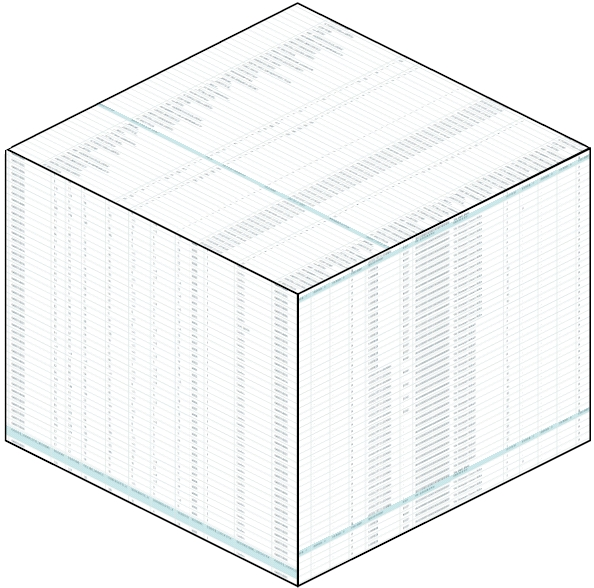
\includegraphics[scale=0.4]{cubo.jpg}
		\caption{Schema \textit{MOLAP}.}
		\label{fig:cubo1}
	\end{figure}
	
	L'alimentazione del DW consiste invece nel mantenere aggiornato il Data Warehouse nel tempo (in genere ad intervalli stabiliti). Per alimentare il Data Warehouse occorre utilizzare il \textit{job} descritto in Sezione \ref{sec:job}. Quindi dopo un primo caricamento, verrà eseguito il \textit{job} ad intervalli regolari (ad esempio ogni anno) con input il \textit{dataset} del bilancio annuale, così da inserire nel Data Warehouse dati sempre aggiornati e permettere analisi più dettagliate ed aggiornate. L'unico requisito richiesto è che i \textit{dataset} dei bilanci annuali dovranno essere già stati ripuliti e validati, così da richiedere a Pentaho di eseguire le trasformazioni necessarie per produrre una struttura compatibile con le precedenti.

